% Selena Gomez 0.0 ['songwriter', 'record producer', 'child actor', 'singer', 'film producer', 'film actor', 'model', 'actor', 'television actor', 'voice actor', 'fashion designer']
% Taylor Swift 0.0035083569 ['lyricist', 'songwriter', 'record producer', 'singer', 'actor', 'public figure', 'recording artist', 'singer-songwriter', 'composer', 'pianist', 'guitarist', 'philanthropist', 'film actor', 'banjoist', 'television actor', 'voice actor']
% 50 Cent 0.0035479667 ['businessperson', 'songwriter', 'investor', 'rapper', 'boxing promoter', 'record producer', 'singer', 'film producer', 'film director', 'singer-songwriter', 'television producer', 'composer', 'entrepreneur', 'film actor', 'executive producer', 'manufacturer', 'screenwriter', 'actor', 'television actor']
% Miley Cyrus 0.0035744922 ['singer', 'singer-songwriter', 'film actor', 'musician', 'actor', 'television actor', 'voice actor']
% Halsey 0.0036942514 ['singer', 'songwriter', 'voice actor']
% Jay-Z 0.0037367728 ['businessperson', 'songwriter', 'investor', 'rapper', 'record producer', 'sports agent', 'singer', 'film producer', 'music executive', 'film director', 'composer', 'television producer', 'entrepreneur', 'philanthropist', 'drug trafficker', 'actor', 'fashion designer']
% Christina Aguilera 0.0038243192 ['music video director', 'songwriter', 'entrepreneur', 'musician', 'television personality', 'diplomat', 'record producer', 'recording artist', 'child singer', 'television actor', 'stage actor', 'dancer', 'singer-songwriter', 'film actor', 'model', 'manufacturer', 'voice actor', 'singer', 'film producer', 'composer', 'actor']
% Kid Cudi 0.0038339603 ['record producer', 'rapper', 'singer', 'singer-songwriter', 'composer', 'guitarist', 'film actor', 'musician', 'actor', 'television actor']
% The Notorious B.I.G. 0.0040764036 ['songwriter', 'rapper']
% Camila Cabello 0.004126276 ['singer', 'songwriter']

\begin{figure*}%
    \centering
    \subfloat{{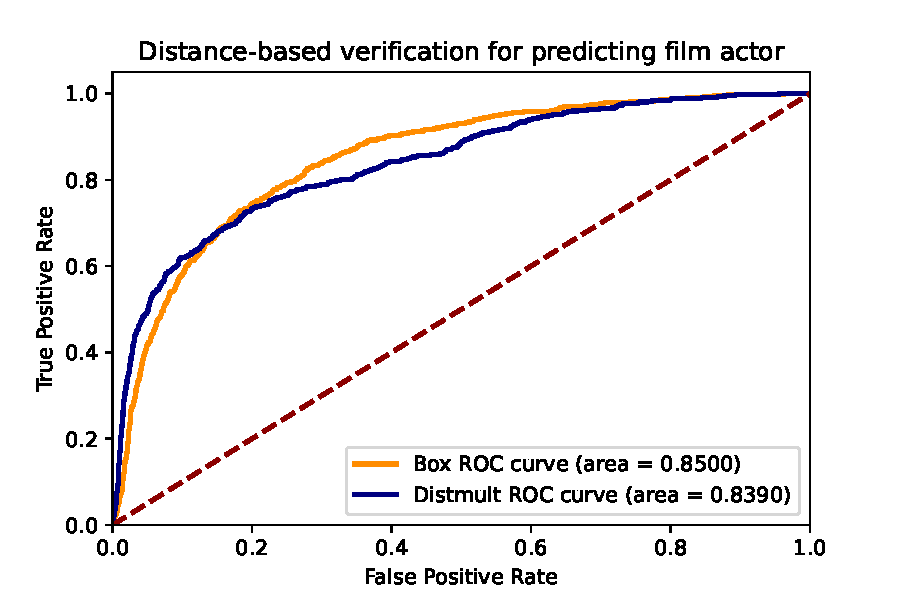
\includegraphics[width=0.65\columnwidth]{submissions/Ali2023/figures/roc_screenwriter-film_actor_dist.pdf} }}%
    \subfloat{{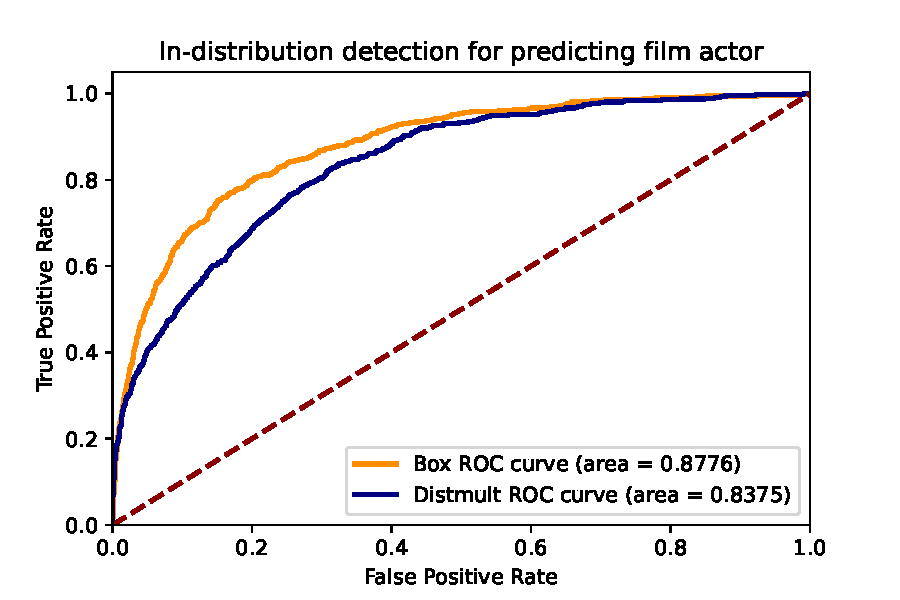
\includegraphics[width=0.65\columnwidth]{submissions/Ali2023/figures/roc_screenwriter-film_actor_in.pdf} }}%
    \subfloat{{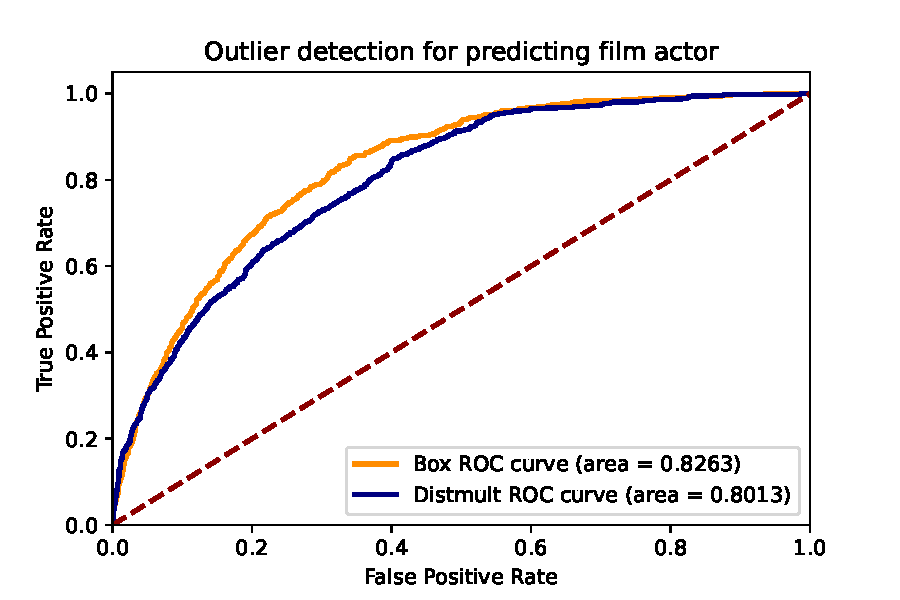
\includegraphics[width=0.65\columnwidth]{submissions/Ali2023/figures/roc_screenwriter-film_actor_out.pdf} }}%
    
    \subfloat{{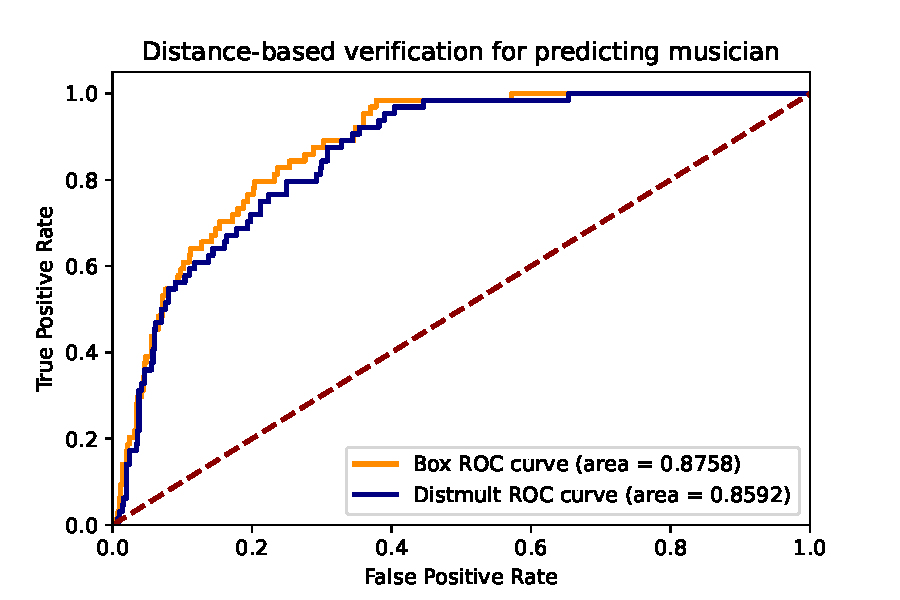
\includegraphics[width=0.65\columnwidth]{submissions/Ali2023/figures/roc_actor-musician_dist.pdf} }}%
    \subfloat{{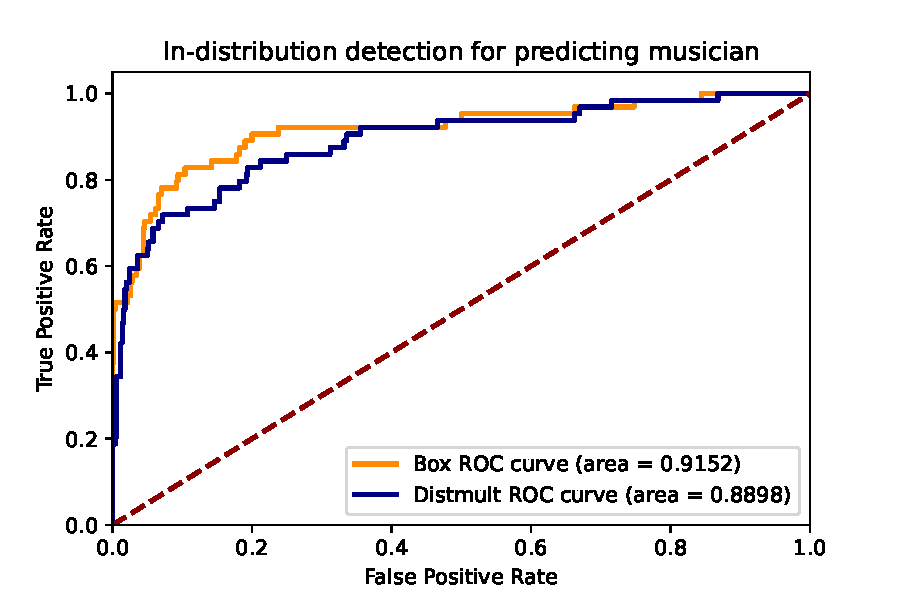
\includegraphics[width=0.65\columnwidth]{submissions/Ali2023/figures/roc_actor-musician_in.pdf} }}%
    \subfloat{{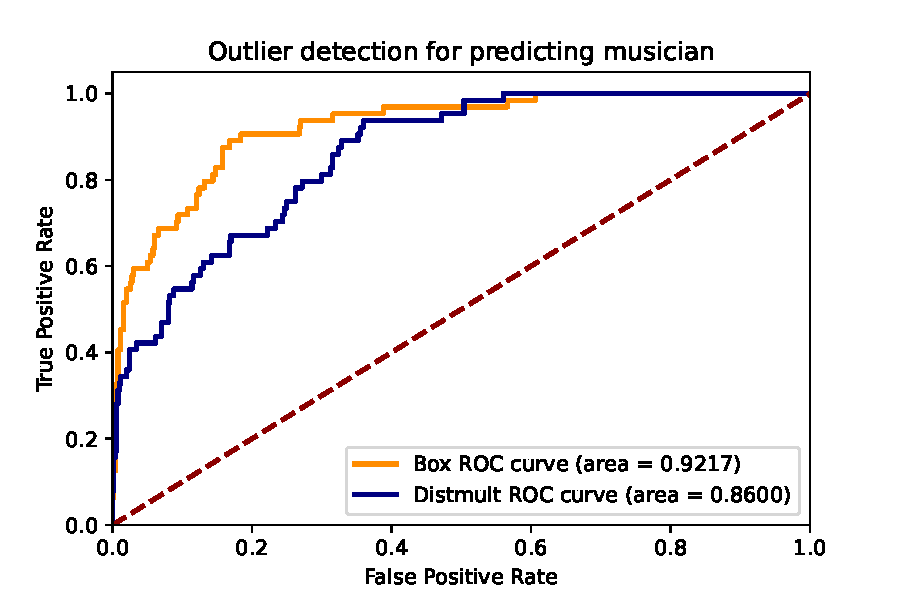
\includegraphics[width=0.65\columnwidth]{submissions/Ali2023/figures/roc_actor-musician_out.pdf} }}%
    
    \subfloat{{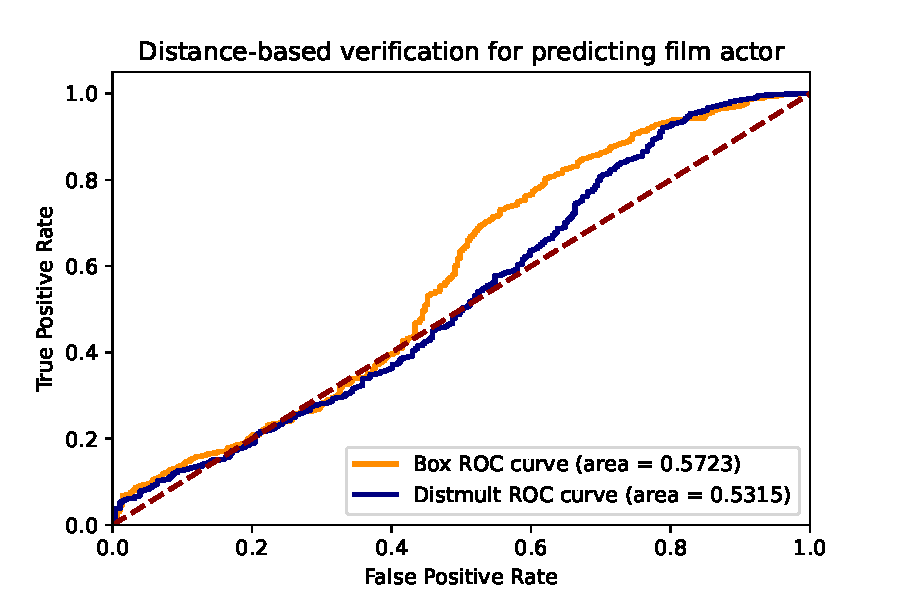
\includegraphics[width=0.65\columnwidth]{submissions/Ali2023/figures/roc_tv_actor-film_actor_dist.pdf} }}%
    \subfloat{{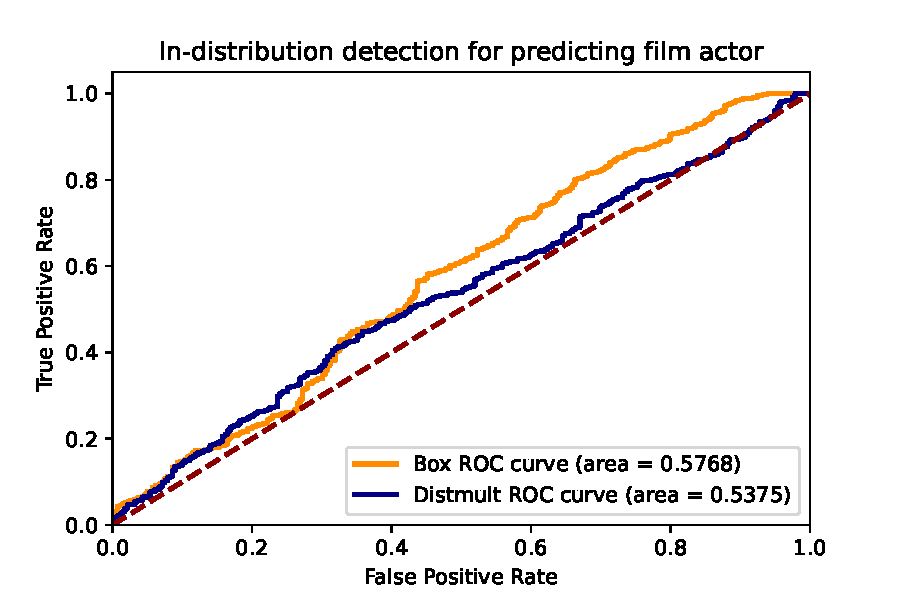
\includegraphics[width=0.65\columnwidth]{submissions/Ali2023/figures/roc_tv_actor-film_actor_in.pdf} }}%
    \subfloat{{\includegraphics[width=0.65\columnwidth]{submissions/Ali2023/figures/roc_tv_actor-film_actor_out.pdf} }}%
    \caption{ROC-AUC curve of Query2box and DistMult in three case studies in fact verification. Query2box consistently achieves better performance than DistMult across cases and metrics.}
    \label{fig:roc-verification}%
\end{figure*}


\begin{figure*}%
    \centering
    \subfloat[\centering label 1]{{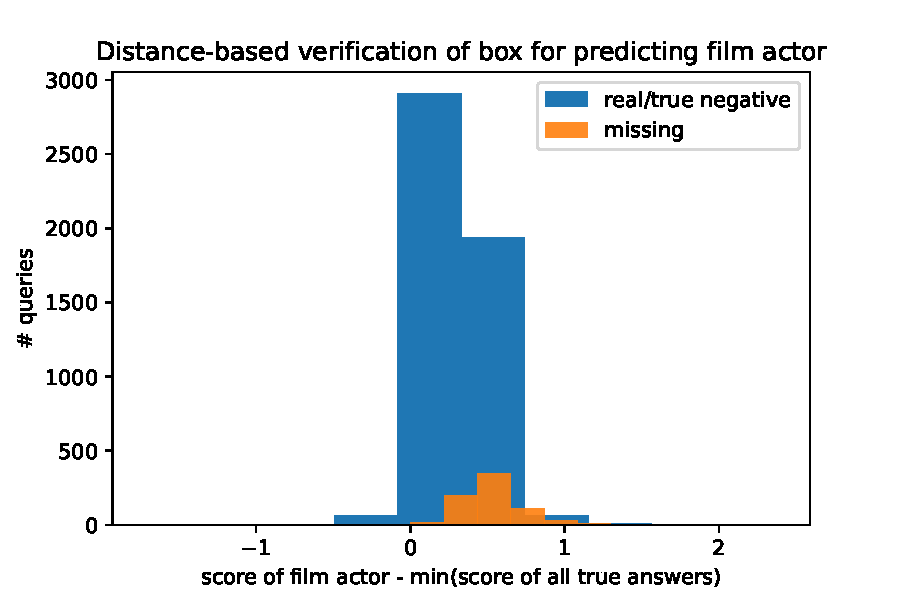
\includegraphics[width=0.65\columnwidth]{submissions/Ali2023/figures/box_screenwriter-film_actor_dist.pdf} }}%
    \subfloat[\centering label 2]{{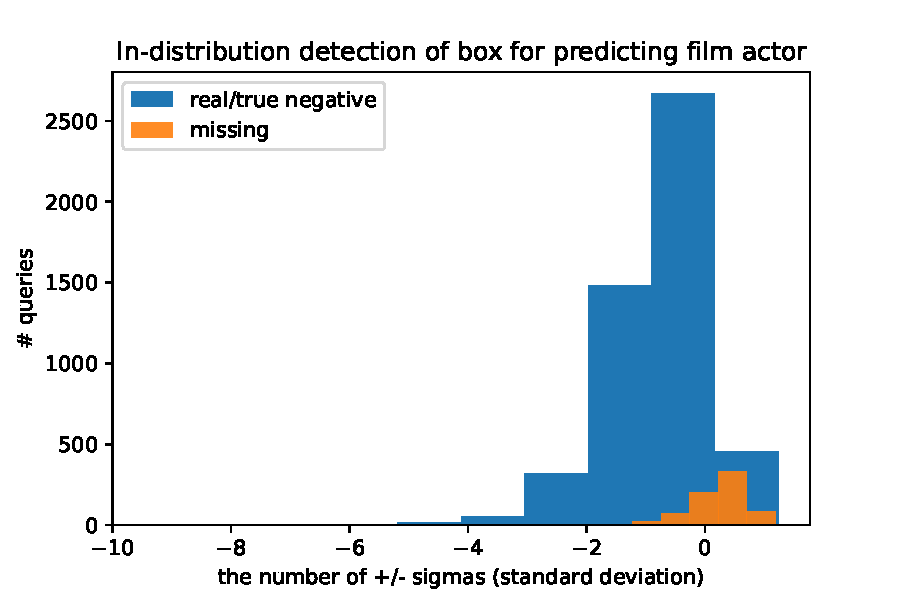
\includegraphics[width=0.65\columnwidth]{submissions/Ali2023/figures/box_screenwriter-film_actor_in.pdf} }}%
    \subfloat[\centering label 2]{{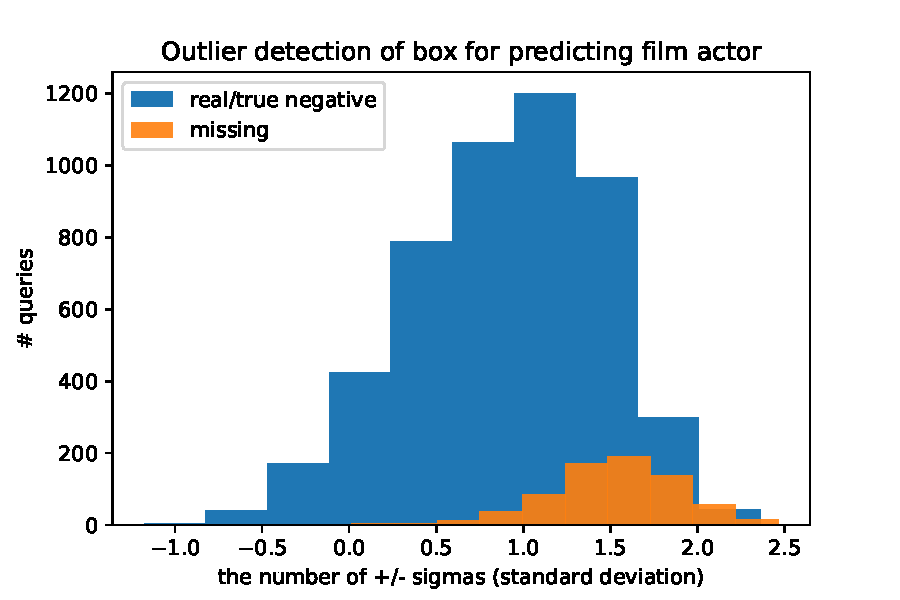
\includegraphics[width=0.65\columnwidth]{submissions/Ali2023/figures/box_screenwriter-film_actor_out.pdf} }}%
    
    \subfloat[\centering label 1]{{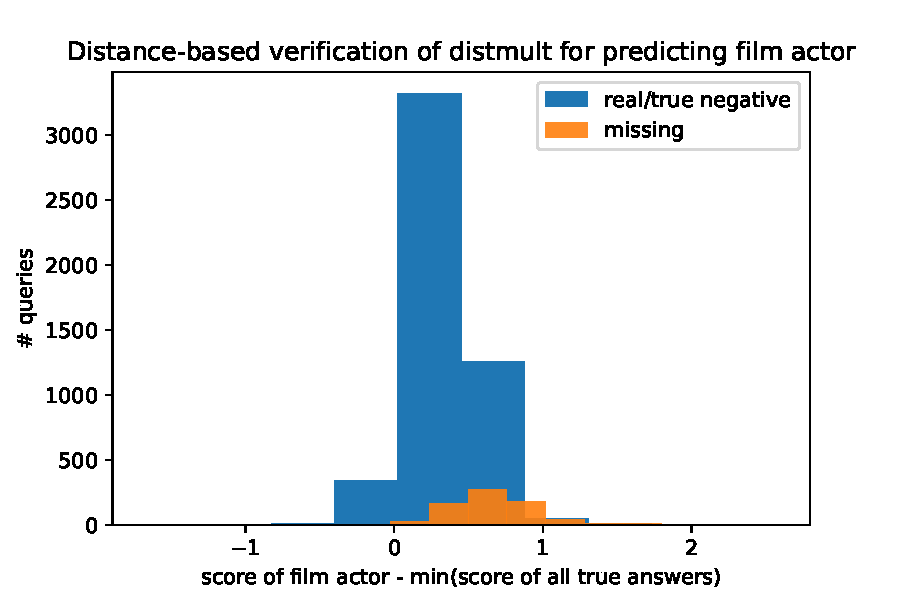
\includegraphics[width=0.65\columnwidth]{submissions/Ali2023/figures/distmult_screenwriter-film_actor_dist.pdf} }}%
    \subfloat[\centering label 2]{{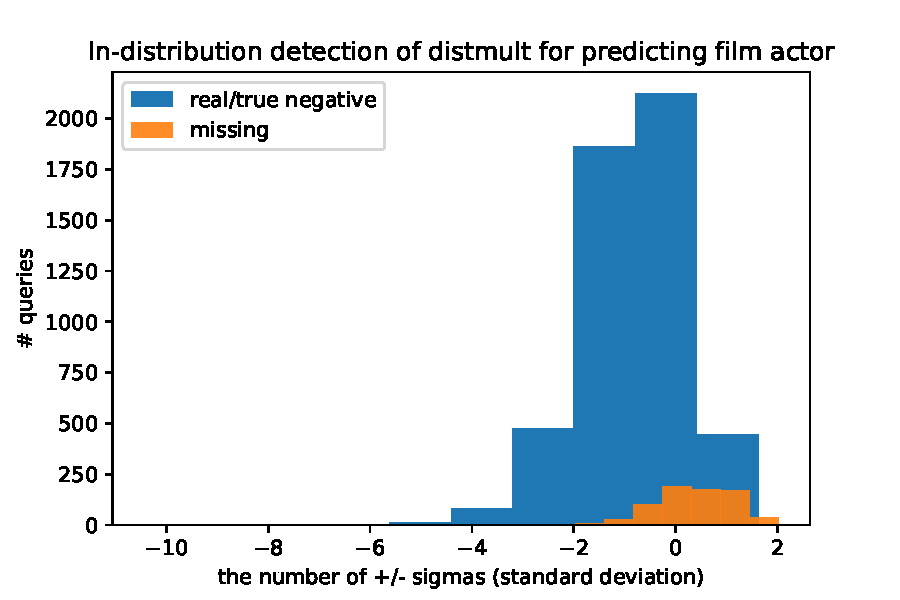
\includegraphics[width=0.65\columnwidth]{submissions/Ali2023/figures/distmult_screenwriter-film_actor_in.pdf} }}%
    \subfloat[\centering label 2]{{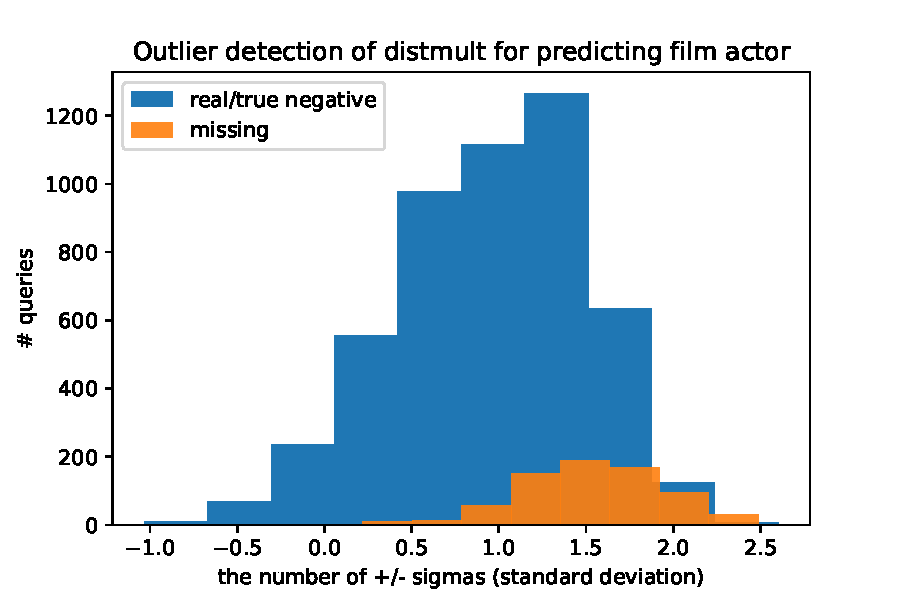
\includegraphics[width=0.65\columnwidth]{submissions/Ali2023/figures/distmult_screenwriter-film_actor_out.pdf} }}%
    \label{fig:example}%
\end{figure*}

%%%%%%%%%%%%%%%%%%%%%%%%%%%%%%%%%%%%%%%%%%%%%%%%%%%%%%%%
% he difference between the score of occupation $B$ and the minimum of score of existing occupations of $v_h$, we measure whether the difference in score can be used to prioritize the fact $(v_h, \texttt{OccupationOf}, B)$; (2) we estimate a Gaussian distribution using the score of existing occupations of $v_h$, then we perform an \emph{in-distribution detection}, \ie, if $B$ is sampled from the Gaussian distribution, then we consider $(v_h, \texttt{OccupationOf}, B)$ a promising missing fact for human curators to verify; (3) we estimate a Gaussian distribution using the score of non-existing occupations of $v_h$, then we perform an \emph{out-of-distribution detection}, \ie, if $B$ is not a sample from the Gaussian distribution we estimated, we prioritize $(v_h, \texttt{OccupationOf}, B)$ and let human curators check it first.  
%%%%%%%%%%%%%%%%%%%%%%%%%%%%%%%%%%%%%%%%%%%%%%%%%%%%%%%%

% \begin{figure}[htp]

% \subfloat{%
%   \includegraphics[clip,width=0.45\columnwidth]{submissions/Ali2023/figures/screenwriter_actor_dist.pdf}%
% }

% \subfloat{%
%   \includegraphics[clip,width=0.45\columnwidth]{submissions/Ali2023/figures/screenwriter_actor_in.pdf}%
% }
% \caption{.}

% \label{fig:verification}

% \end{figure}

\subsubsection{Design choice for related facts}
\paragraph{Non-existing facts with same head entity $v_h^i$ and relation $r_i$}
The first intuition is that we can collect a pool of non-existing fact triplets with the same head entity and relation for the triplet $(v_h^i, r^i, v_t^i)$ to verify. Then we may compare the distance of $(v_h^i, r^i, v_t^i)$ (calculated using \eqref{eq:kgelossfunc}) and the distribution of distance of those non-existing fact triplets. We may score the triplet $(v_h^i, r^i, v_t^i)$ by checking whether this is an ``outlier'' to the pool of non-existing facts. If it is an outlier, we may prioritize this triplet fact since it is more likely to be a missing fact.
% from a set of non-existing facts. In such away we can formulate the missing fact imputation task as out-of-distribution sample detection task. If the triplet to verify is detected as an outlier to the pool of non-existing facts, then we prioritize this triplet fact since it is more likely to be a missing fact.
In detail, for each triplet in the given set of triplets $\{(v_h^1, r^1, v_t^1), \dots, (v_h^n, r^n, v_t^n)\}$ to verify, we score it in the following way against a set of related non-existing facts.
In order to score $(v_h^i, r^i, v_t^i)$, we first construct non-existing facts by replacing the tails of the query $(v_h^i, r^i, ?)$. We randomly sample entities $v$ from KG as the tail if $(v_h^i, r_i, v) \notin \gE$. This is sufficient in our use case and achieves empirically nice experimental results (detailed in \Secref{sec:experiment}), but one could design better negative sampling strategies \tocite{} to further improve fact pool. 
Assume we sample $k$ non-existing facts for the $i$-th triplet $(v_h^i, r^i, v_t^i)$: $\{(v_h^i, r^i, v_1), \dots, (v_h^i, r^i, v_k)\}$ as well as the triplet fact $(v_h^i, r^i, v_t^i)$ to verify, we formulate and measure the delta using the distance calculated by the embeddings, \ie, we calculate the distance $d_1=\distt{v_h^i}{r^i}{v_1}, \dots, d_k, d_t=\distt{v_h^i}{r^i}{v_t^i}$, and measure whether $d_t$ is an out-of-distribution sample to $\{d_1, \dots, d_k\}$. Inspired by \tocite{a simple unified framework}, we estimate a Gaussian distribution $\gN_\text{NE}=(\mu_\text{NE}, \sigma_\text{NE})$ over the distances of non-existing facts $\{d_1, \dots, d_k\}$, and score the triplet $(v_h^i, r^i, v_t^i)$ by calculating how many standard deviations $d_t$ are away from the mean: $s_i=\frac{d_t - \mu_\text{NE}}{\sigma_\text{NE}}$. In order to identify the promising triplet facts, we may formulate the problem as a binary classification task using the $s_i$, and prioritize ones with small $s_i$, which means that they are far from the $\mu_\text{NE}$ and likely to be a missing fact.
Since large-scale KGs (with tens of millions of nodes and hundreds of millions of edges) are often extremely sparse, we can easily construct pool of $k$ non-existing facts with $k>1000$. In such a way, we can have an accurate estimation of the distribution $\gN_\text{NE}$.

\paragraph{Existing facts with same head entity $v_h^i$ and relation $r_i$}
We can also approach the problem from the opposite perspective. Instead of calculating the delta using a set of non-existing facts, we can score the triplet fact to verify using a set of existing facts with the same head entity $v_h$ and relation $r_i$.  
For a given $(v_h^i, r^i, v_t^i)$, we find all the answers $\gA_q$ of query $q=(v_h^i, r^i, ?)$ from the given KG, and define the related triple facts to be $\{(v_h^i, r^i, v_1), \dots, (v_h^i, r^i, v_k)\}$, where $v_1, \dots, v_k\in\gA_q$. Similarly, we may calculate the distance for all existing triplet facts $d_1=\distt{v_h^i}{r^i}{v_1}, \dots, d_k=\distt{v_h^i}{r^i}{v_k}, d_t=\distt{v_h^i}{r^i}{v_t^i}$. Then we can estimate a Gaussian distribution over $\{d_1, \dots, d_k\}$: $\gN_\text{E}=(\mu_\text{E}, \sigma_\text{E})$, and score the triplet fact $(v_h^i, r^i, v_t^i)$ with the number of standard deviations from the mean: $s_i=\frac{d_t - \mu_\text{E}}{\sigma_\text{E}}$. 
However, the key challenge of this modeling is that the estimation has high variance due to the limited number of answer size $|\gA_q|$. Below we improve the estimation accuracy by loosening the definition of related triple facts for $(v_h^i, r^i, v_t^i)$.

\paragraph{Existing facts with close head entities and relation $r_i$}
In order to combat the small number of existing related facts for a triplet fact $(v_h^i, r^i, v_t^i)$ to verify, we relax the definition of related existing facts by finding entities $v$ that are close to the head entity $v_h^i$ in the embedding space. The intuition is that with the pretrained KG embedding, close entities share similar semantic meaning, \eg, the neighbors of Selena Gomez are all singers \todo{add a figure or table to show this}. Assume we find $m$ close entities of $v_h^i$: $\{v_1, \dots, v_m\}$, we collect the pool of existing related facts $\cup_{j=1}^m\:\{(v_j, r_i, v) | v\in\gA_q, q=(v_j, r_i, ?)\}$. Then we use the same framework to score the triplet fact to verify with the number of standard deviations away from the new mean. We can tune the parameter $m$ to achieve a balance between computation efficiency and the accuracy of the estimation.

\paragraph{Extension to Mahalanobis distance}
All the above methods aim to derive a confidence score $s_i$ by estimating a Gaussian distribution over a set of scalar distances $\{d_1, \dots, d_k\}, d_i\in\R$. However, most KG embeddings are high dimensional and the distance of each dimension is calculated separately in many shallow KG embedding models, \eg, TransE (w/ L1 distance), DistMult, \etc, as well as multi-hop KG embedding models, \eg, Query2box. Thus, an alternative is to obtain a high-dimension vector that comprises the distance along each dimension. In detail, if we use the TransE model, the distance vector for a triplet fact $(v_h, r, v_t)$ is $\vd=f_\theta(v_h)+f_\theta(r)-f_\theta(v_t)$. Given a fact to verify $(v_h^i, r^i, v_t^i)$ and a corresponding pool of facts $\{(v_h^i, r^i, v_1), \dots, (v_h^i, r^i, v_k)\}$, we can calculate the high dimensional distance vector $\{\vd_1, \dots, \vd_k\}$ and estimate a mean and covariance matrix from the set.
\begin{align}
    \vmu&=\frac{1}{k} \sum_j \vd_j \nonumber\\
    \mSigma&=\frac{1}{k} \sum_j (\vd_j - \vmu)(\vd_j - \vmu)^\intercal.
\end{align}
Now we can score the triplet $(v_h^i, r^i, v_t^i)$ with $s_i = $

\paragraph{Application to verification of existing facts}
Above we introduce how we use our framework to solve one of the fact verification tasks, namely identifying the likely missing triplet facts. Another task that falls within the same domain is that we want to prioritize the existing triplet facts on the graph that are likely to be False. Our framework can be naturally adapted for this setting, where we can still collect related triplet facts, estimate a distribution of distance, and calculate how many standard deviations is this triplet fact away from the mean. Then we can use this score to identify and prioritize promising triplet facts in this setting.